% !TEX program = pdflatex
% Factor crowding and factor decay in China's A-share market: FRL submission manuscript.
% Positioning: measurement comparison and boundary analysis, not a single-country replication.
% Revised 2026-10-24: timing, faithful weekly comomentum, and long-horizon risk checks.
% Auxiliary results: scripts 19--23 and corresponding reports/CSV files.
% Author-year bibliography style required by the current FRL guide: elsarticle-harv.
\documentclass[final,1p,authoryear]{elsarticle}

\usepackage{amsmath,amssymb}
\usepackage{newtxtext,newtxmath}
\usepackage{xcolor}
\usepackage{booktabs}
\usepackage{graphicx}
\usepackage{threeparttable}
\usepackage{adjustbox}
\usepackage[section]{placeins}
\usepackage[hidelinks]{hyperref}
\hypersetup{pdftitle={Measuring Factor Crowding When Leverage Is Observable: Evidence from China's A-Share Market},pdfauthor={Jiaheng Wen}}
\usepackage{xurl}
\emergencystretch=1em


\journal{Finance Research Letters}

\begin{document}

\begin{frontmatter}

\title{Measuring Factor Crowding When Leverage Is Observable:
       Evidence from China's A-Share Market}

\author[tongji]{Jiaheng Wen\corref{cor}}
\cortext[cor]{Corresponding author.}
\ead{2790443124@qq.com}
\address[tongji]{Tongji University, Shanghai, China}

\begin{abstract}
Factor crowding is difficult to measure because holdings are rarely observed and return-based proxies may capture several forms of common movement. We compare residual-return comovement with an observable margin-financing-balance proxy for six style factors in China's A-share market from 2015--2025. Within-factor comovement between the measures is limited. The margin-balance proxy is conditionally negatively associated with subsequent factor returns after controlling for factor momentum, balance levels, long- and short-leg coverage, and factor fixed effects. In the main six-month specification, a one-standard-deviation increase is associated with a 5.2-percentage-point lower horizon-sum return. The association is concentrated in the low-side leg, although subsample and factor-specific estimates are not uniformly significant. Comomentum gives more heterogeneous evidence: a closer weekly Lou--Polk analogue is negatively associated with 12-month compounded momentum returns, but pooled significance is construction-dependent and the association does not survive the strictest multiple-testing corrections. Long-horizon skewness results also vary between pooled factors and momentum alone. Because rolling formation and holding windows overlap, we use pooled circular-shift permutation inference alongside HAC standard errors. The results support a measurement distinction rather than a universal crowding effect: return comovement and leveraged financing are not interchangeable proxies, and all evidence is associational rather than causal.
\end{abstract}

\begin{keyword}
factor crowding \sep{} factor decay \sep{} comomentum \sep{} margin financing \sep{} China \sep{} A-share market
\end{keyword}
\noindent\textbf{JEL classification:} G12.

\end{frontmatter}

% ============================================================
\section{Introduction}

\noindent Capital flowing into a factor strategy can eliminate the mispricing it exploits and leave
crowded trades exposed to reversal \citep{shleifer1997limits,delong1990noise,stein2009presidential,barberis2003style}.
The empirical obstacle is measurement: positions are usually unobserved, while returns also
contain the price pressure that crowding creates. The \emph{comomentum} measure of
\citet{lou2022comomentum} infers common positioning from residual-return correlations and predicts
lower US momentum returns, higher volatility, and more negative skewness.

We compare this indirect proxy with observable margin-financing balances in China's A-share
market, where margin-financing arrangements and short-sale eligibility differ from the US setting.
The contribution is a measurement comparison, not a single-country replication or a claim to
observe total positions. Using six factors over 2015--2025, we find limited comovement between
the proxies. Margin balances are negatively associated with pooled future returns; comomentum
results vary by horizon, construction, and factor. Neither is uniformly predictive.

Three design concerns are central. Balance changes mechanically contain balance-level
information, so we control for that level. Factors with strong past returns may attract
financing, so we include and orthogonalise against factor momentum and estimate factor-specific
slopes. Finally, overlapping formation and holding windows motivate pooled circular-shift
permutation inference with the same estimator used for the observed statistic. These choices
connect the paper to work on factor decay and crowding \citep{mclean2016does,beck2016will,
lou2022comomentum} and Chinese margin trading \citep{bian2026drivers,xing2026pmo}.

\section{Data and methodology}
% ============================================================

\subsection{Data}

\noindent We use the full A-share cross-section from January 2015 to December 2025. Daily prices,
trading volumes, turnover, and point-in-time valuation ratios are from Baostock
(www.baostock.com); the
universe includes delisted firms. The cleaned universe contains 5{,}418 stocks over 2{,}674
trading days. After retaining historical ST trading days and filtering ST status only at
formation, the monthly panel covers 5{,}248 stocks. Individual-stock
margin-financing balances, covering the designated margin-eligible list, are from the Shanghai
and Shenzhen exchanges.

Signals use only information available by month-end, with next-trading-day balance availability.
A stratified 40-stock audit supports disclosure-date updating of the valuation fields, without
ruling out later revisions. At formation, we exclude stocks that are suspended, ST, financial,
or listed for less than 180 days, as well as stock-months with more than ten non-trading days. Industry classification is a current snapshot, a limitation. Portfolios use the full
cross-section; expanding margin eligibility affects only the financing proxy, for which we
retain coverage controls.

Monthly factors are value (book-to-market), size (negative log float capitalisation), momentum
(months $t-12$ to $t-1$), quality (price-to-book divided by trailing price-to-earnings), low
volatility (negative prior 60-day volatility), and turnover (negative prior 20-day turnover).
Decile membership and float-capitalisation weights are frozen at formation; stocks not trading
on the market month-end use their last observed in-month snapshot. At realisation, weights are
renormalised over non-missing next-month returns without assigning missing returns a zero.
Historical and holding-period ST trading days remain in return construction. A separate raw-daily
audit independently verifies this convention and distinguishes observable realisations,
in-holding-month terminal events, nonterminal gaps, and sample-end right censoring.
Returns are top minus bottom deciles; common-month-end, daily-leg, and terminal-return
sensitivities isolate the resulting timing and estimator choices.

\subsection{Two measures of crowding}

\paragraph{Indirect: comomentum.}
For each factor's long and short deciles, the baseline averages sampled pairwise correlations
of daily residuals from a local three-factor model over 250 trading days, capping each leg at
100 stocks with a fixed seed. It is a daily variant, not an exact Lou--Polk replication.
A sampling audit repeats the full measure and specification-D inference for 20 predeclared seeds,
including the production seed, without pooling seed replicates or selecting by significance.
Auxiliary weekly analogues use 52 Friday-to-Friday industry-adjusted returns and correlations
with the leave-one-out equal-weighted leg portfolio. Variants require complete histories and
impose local price/size screens. Current-snapshot industries and the local benchmark preclude
a literal US replication.

\paragraph{Margin-financing-balance proxy.}
We aggregate $\Delta MB_{i,t}/MV_{i,t}$ within each leg using formation float-capitalisation
weights and subtract the short-leg aggregate from the long-leg aggregate. Snapshots older than
45 calendar days and unavailable lagged snapshots are missing, never zero changes. Intensities
are renormalised over valid observations; coverage uses the full formation leg. Size's long-leg
coverage is especially thin (mean 0.26 versus 0.82--0.93 elsewhere), motivating two-leg coverage
controls and coverage-floor checks. This observable financing proxy is neither an account-level
position nor a pure flow.

\subsection{Empirical design}

\noindent For each measure $C_{f,t}$ and horizon $h \in \{1,3,6,12\}$ we estimate
\begin{equation}
R^{f}_{t \to t+h} \;=\; \alpha_f \;+\; \beta\, C_{f,t} \;+\; \gamma' X_{f,t} \;+\; \varepsilon_{f,t},
\end{equation}
where $R^{f}_{t\to t+h}$ sums the next $h$ monthly long-short returns from $t+1$, $\alpha_f$
is a factor fixed effect, and $X$ contains past 1-, 6-, and 12-month factor returns, margin
level, and two-leg coverage. Auxiliary tests use compounded returns. Newey--West lags are six
in primary and twelve in long-horizon specifications; six factor clusters cannot support reliable
cluster asymptotics. We also orthogonalise the proxy against past returns and estimate separate
factor slopes.

Circular shifts within factor preserve the controls, sample, estimator, and HAC lag length.
Reported finite-permutation $p$-values use $(1+B_{\geq})/(1+B)$. Synthetic-null and block-bootstrap
power checks accompany the replication. Auxiliary construction and factor families include
Benjamini--Hochberg and Bonferroni corrections; individual slopes are exploratory. Primary tests
use both baseline proxies at $h\in\{1,3,6\}$; horizon 12, alternative constructions, and risk
outcomes remain auxiliary.

% ============================================================
\section{Results}

\subsection{The two measures of crowding are only weakly related}

\noindent The two measures have limited linear comovement: within-factor correlations range from
$-0.28$ for value (and $-0.15$ for turnover) to $+0.25$ for size, and are near zero for
quality and low volatility. Pooling the six factors gives $-0.13$, or $-0.07$ after removing
factor-specific means. Across the 20 seeds, the factor-demeaned pooled Pearson correlation
ranges from $-0.095$ to $-0.035$; the quality-factor Spearman correlations and the
low-volatility-factor correlations can cross zero.
These correlations may also reflect timing, coverage, nonlinear dependence, or sampling noise.
Figure~\ref{fig:series} plots both series for each factor.

\begin{figure}[htbp]\centering
\IfFileExists{figures/fig_crowding_series.pdf}{%
  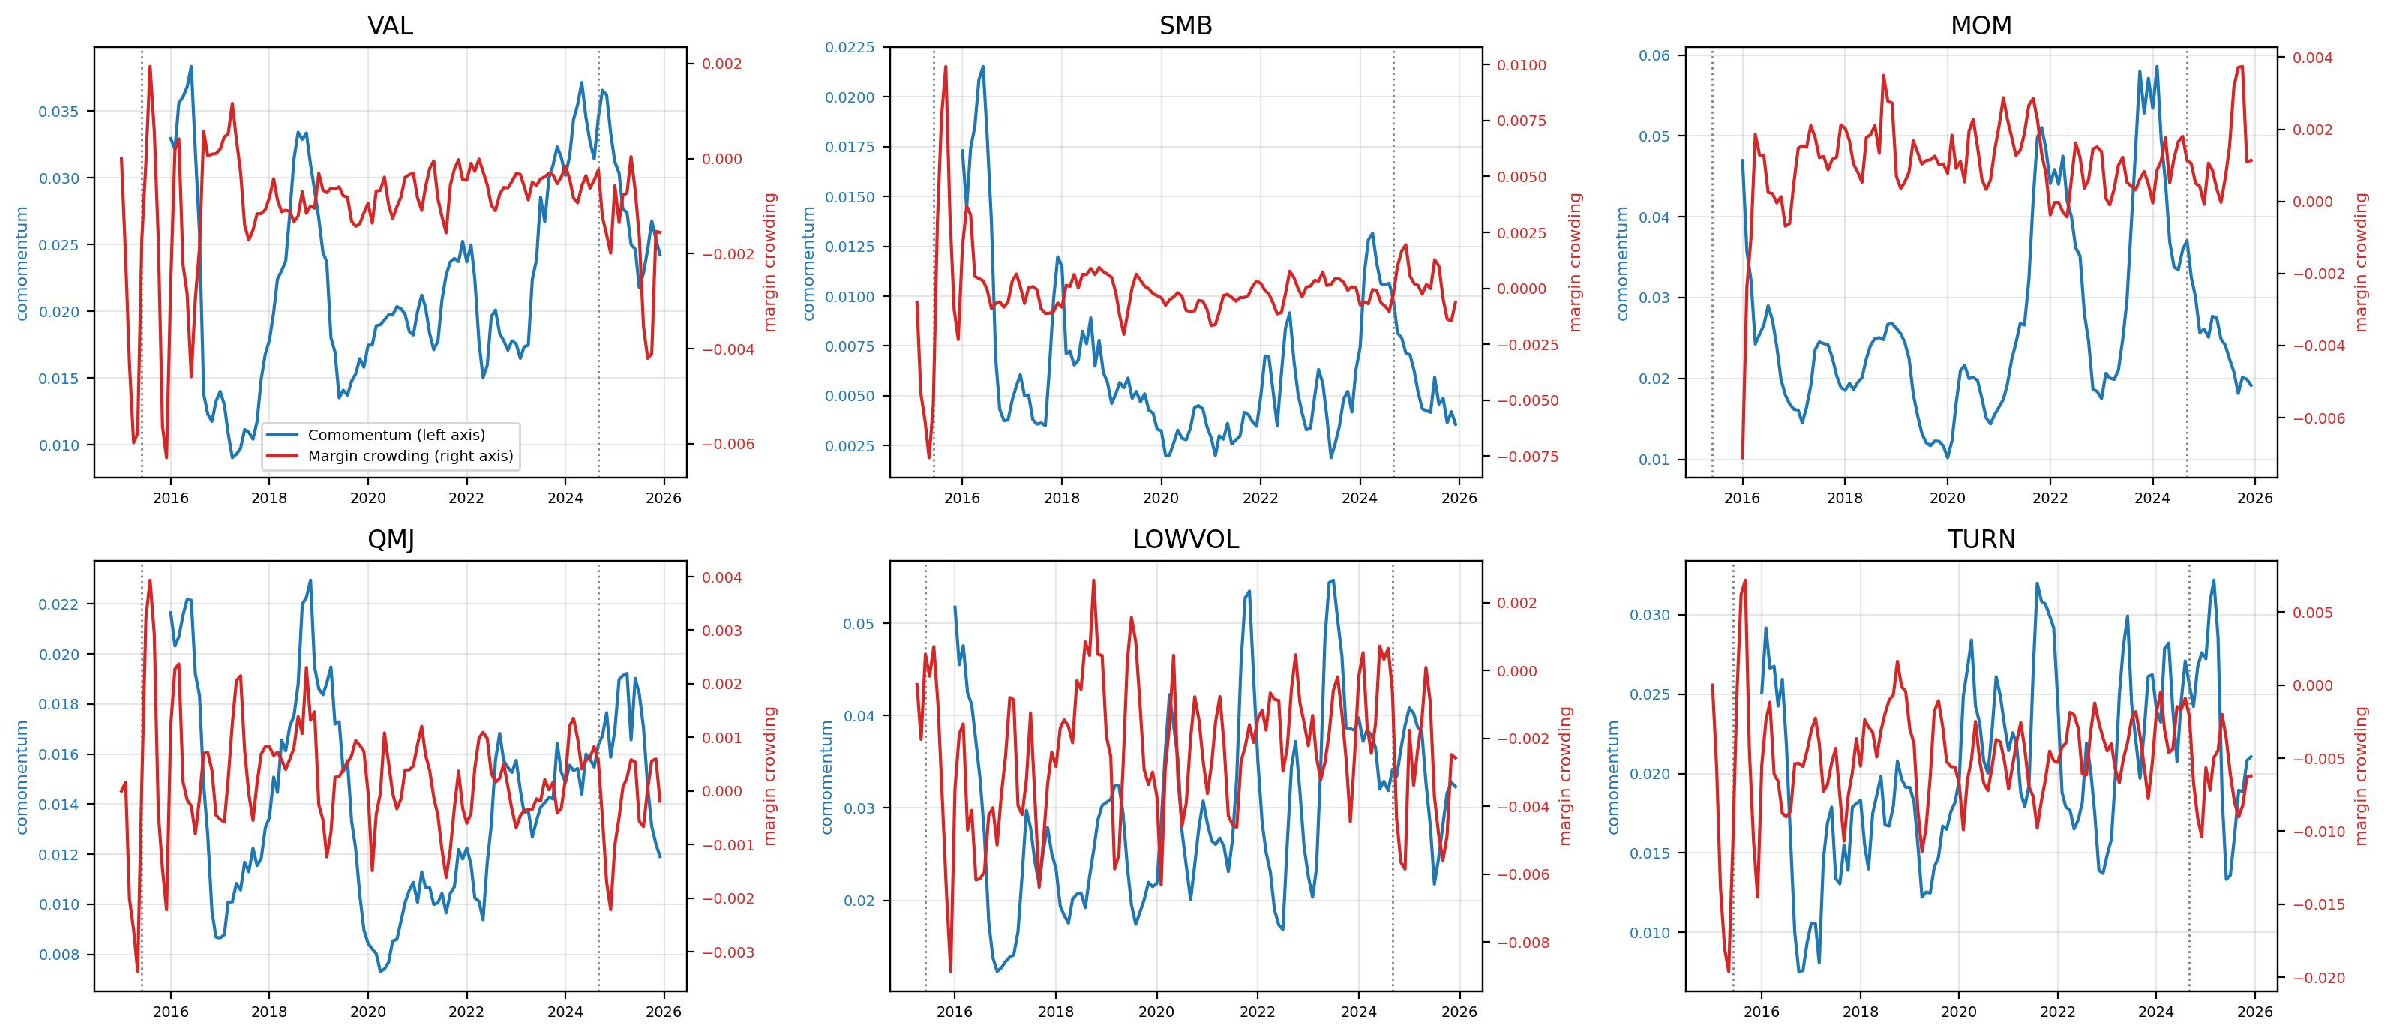
\includegraphics[width=\textwidth]{figures/fig_crowding_series.pdf}%
}{%
  \fbox{\parbox{0.9\textwidth}{\centering Figure 1 unavailable}}
}
\caption{Crowding measures by factor (three-month rolling means). Baseline comomentum
(blue, left axis) and margin crowding (red, right axis) use different scales. Dotted lines
mark June 2015 and September 2024.}
\label{fig:series}
\end{figure}


\subsection{Return predictability differs by proxy, horizon, and factor}

\noindent At one, three, and six months, baseline daily comomentum has no robust return association
(Table~\ref{tab:main}). Across all 20 sampling seeds these coefficients remain positive; six-month
permutation $p$-values range from $0.265$ to $0.667$, with no seed below $0.10$.
Margin balances are negatively associated with returns. Adding factor
momentum, balance level, and two-leg coverage strengthens rather than removes the association:
the six-month coefficient changes from $-0.0447$ with momentum controls to $-0.0524$ in
specification D (permutation $p=0.010$).

\begin{table}[htbp]\centering
\caption{Crowding and future factor returns}
\label{tab:main}
\begingroup\small\setlength{\tabcolsep}{3pt}
\begin{tabular}{llcccc}
\toprule
\multicolumn{6}{l}{\textit{Coefficient (stars from permutation $p$)}} \\
Measure & $h$ & A & B & C & D \\
\midrule
Comomentum & 1 & 0.0019 & 0.0021 & 0.0031 & 0.0036 \\
Comomentum & 3 & 0.0011 & 0.0037 & 0.0068 & 0.0082 \\
Comomentum & 6 & 0.0014 & 0.0059 & 0.0113 & 0.0131 \\
Comomentum & 12 & -0.0211 & -0.0183 & -0.0107 & -0.0102 \\
Margin-balance proxy & 1 & -0.0087*** & -0.0137*** & -0.0150*** & -0.0157*** \\
Margin-balance proxy & 3 & -0.0115 & -0.0226*** & -0.0264*** & -0.0284*** \\
Margin-balance proxy & 6 & -0.0177 & -0.0338*** & -0.0383*** & -0.0400*** \\
Margin-balance proxy & 12 & -0.0190 & -0.0377* & -0.0469** & -0.0479** \\
\midrule
\multicolumn{6}{l}{\footnotesize Notes: Stars use finite circular-shift permutation $p$-values; * $p<0.10$, ** $p<0.05$, *** $p<0.01$.} \\
\bottomrule
\end{tabular}

\endgroup
\end{table}

The magnitude is economically material: in specification D at $h=6$, a one-standard-deviation
increase in the margin-balance proxy accompanies approximately a $5.2$ percentage point lower
horizon-sum long-short return over six months ($4.4$ points per within-factor standard deviation).
At $h=12$, the compounded-return specification gives $\beta=-0.0709$ with HAC(12) and permutation
$p=0.021$. However, the momentum-factor slope is near zero ($p=0.667$), while quality is the
strongest individual contributor ($p=0.009$; six-factor BH $p=0.056$). These are conditional,
heterogeneous associations, not universal or causal effects.

The weekly comomentum analogues qualify the shorter-horizon null rather than overturning it.
For momentum's 12-month compounded return, the weekly leave-one-out measure gives
$\beta=-0.1885$ and permutation $p=0.031$; low volatility gives $p=0.048$. Neither survives
six-factor BH correction (both $p=0.143$), and the seven-construction Bonferroni-adjusted
momentum result is $p=0.219$. Pooled 12-month estimates are also construction-dependent
($p=0.073$ for the core weekly analogue and $0.010$ for its screened version). We therefore
interpret the long-horizon comomentum evidence as exploratory and factor-specific, not as a
general replication of Lou--Polk return predictability.


\subsection{The signal is in the low-side leg}

\noindent Table~\ref{tab:legs} decomposes the six-month association with common specification-D
controls. The long leg contributes little ($\beta=0.0003$, $p=0.990$), whereas the short leg
carries the spread result ($\beta=0.0527$, $p=0.010$). Its own financing intensity also predicts
its own return ($\beta=-0.0608$, $p=0.020$); the long-leg analogue is insignificant ($p=0.196$).
Comomentum shows no corresponding leg pattern.

\begin{table}[htbp]\centering
\caption{Leg decomposition of the crowding association}
\label{tab:legs}
\begingroup\footnotesize\setlength{\tabcolsep}{2pt}
\begin{tabular}{llllcccc}
\toprule
Panel & Measure & Return leg & $h$ & $\beta$ & HAC $t$ & Perm. $p$ & $N$ \\
\midrule
A & Comomentum & Long-short & 6 & 0.0208 & 2.11 & 0.265 & 669 \\
 & Comomentum & Long leg & 6 & 0.0052 & 0.62 & 0.696 & 669 \\
 & Comomentum & Short leg & 6 & -0.0156 & -1.28 & 0.608 & 669 \\
A & Margin-balance proxy & Long-short & 1 & -0.0190** & -3.44 & 0.019 & 699 \\
 & Margin-balance proxy & Long leg & 1 & -0.0020 & -0.64 & 0.533 & 699 \\
 & Margin-balance proxy & Short leg & 1 & 0.0170** & 3.45 & 0.019 & 699 \\
A & Margin-balance proxy & Long-short & 6 & -0.0524*** & -4.32 & 0.010 & 669 \\
 & Margin-balance proxy & Long leg & 6 & 0.0003 & 0.03 & 0.990 & 669 \\
 & Margin-balance proxy & Short leg & 6 & 0.0527*** & 4.40 & 0.010 & 669 \\
\midrule
B & Margin-balance proxy, long leg & Long leg & 1 & -0.0093* & -1.91 & 0.093 & 699 \\
B & Margin-balance proxy, short leg & Short leg & 1 & -0.0253*** & -4.03 & 0.009 & 699 \\
B & Margin-balance proxy, long leg & Long leg & 6 & -0.0184 & -1.61 & 0.196 & 669 \\
B & Margin-balance proxy, short leg & Short leg & 6 & -0.0608** & -3.96 & 0.020 & 669 \\
\midrule
\multicolumn{8}{l}{\parbox{\dimexpr\textwidth-10pt\relax}{\footnotesize Notes: Panel A regresses each leg's horizon-sum return on the total margin-balance or comomentum measure, with the identical controls and sample as specification D, so the long-short coefficient equals the long-leg coefficient minus the short-leg coefficient. Panel B pairs each leg's return with that leg's own financing measure. Stars use finite circular-shift permutation $p$-values; * $p<0.10$, ** $p<0.05$, *** $p<0.01$.}} \\
\bottomrule
\end{tabular}

\endgroup
\end{table}

\newpage

\subsection{Flows versus stocks}

\noindent Flow variants scale monthly financing purchases, or purchases less repayments where
available, by float capitalisation. Purchase flows are significant only at one month; Shanghai
net flows are significant at all four horizons (Table~\ref{tab:flow}). In horse races, purchase
flows add no independent content, while net flows retain content only at six months. Balance
changes correlate 0.546 and 0.540 with the two flows, indicating partly distinct signals.

\begin{table}[htbp]\centering
\caption{Financing flows versus balance changes}
\label{tab:flow}
\begingroup\small\setlength{\tabcolsep}{2.5pt}
\begin{tabular}{llcccc}
\toprule
Measure & $h$ & $\beta$ & HAC $t$ & Perm. $p$ & $N$ \\
\midrule
Financing purchases (buy flow) & 1 & -0.0378** & -2.91 & 0.031 & 644 \\
Financing purchases (buy flow) & 3 & -0.0571* & -2.81 & 0.097 & 632 \\
Financing purchases (buy flow) & 6 & -0.0811 & -2.79 & 0.169 & 614 \\
Financing purchases (buy flow) & 12 & -0.0572 & -1.44 & 0.472 & 578 \\
\midrule
Net financing flows (SSE) & 1 & -0.0178** & -3.43 & 0.016 & 644 \\
Net financing flows (SSE) & 3 & -0.0302** & -3.19 & 0.048 & 632 \\
Net financing flows (SSE) & 6 & -0.0623** & -5.23 & 0.017 & 614 \\
Net financing flows (SSE) & 12 & -0.0529** & -2.33 & 0.019 & 578 \\

\midrule
\multicolumn{6}{l}{\parbox{\dimexpr\textwidth-10pt\relax}{\footnotesize Notes: Both measures are leg-level float-weighted monthly financing intensities (long leg minus short leg) with specification-D controls and the measure's own trailing twelve-month mean as an additional level control; net flows are available for Shanghai only. Stars use finite circular-shift permutation $p$-values; * $p<0.10$, ** $p<0.05$, *** $p<0.01$.}} \\
\bottomrule
\end{tabular}

\endgroup
\end{table}


\subsection{Risk diagnostics are mixed and do not validate either proxy}

\noindent Using common samples and HAC(12), pooled weekly-skewness coefficients for the core weekly
analogue are $-0.0965$ at six months and $-0.0870$ at twelve months (permutation $p=0.010$;
four-measure BH $p=0.020$ and $0.021$). Yet twelve-month daily volatility and bad-week frequency
give $p=0.667$ and $0.188$. For momentum alone, six- and twelve-month weekly-skewness $p$-values
are $0.775$ and $0.729$; only its three-month daily-volatility result is positive ($p=0.010$,
BH $p=0.038$). These mixed diagnostics neither establish a failed implementation nor validate
comomentum as crowded arbitrage trading. Financing likewise lacks a uniform second-moment pattern.


\subsection{Separating crowding from factor momentum}

\noindent Orthogonalising against past returns and margin level leaves the primary margin-balance
association intact (Table~\ref{tab:orth}). Six factor-specific slopes remain exploratory.

\begin{table}[htbp]\centering
\caption{Separating crowding from factor momentum}
\label{tab:orth}
\begingroup\small\setlength{\tabcolsep}{2.5pt}
\begin{tabular}{llcccc}
\toprule
Measure & Layer & $h$ & $\beta$ & HAC $t$ & Perm. $p$ \\
\midrule
Comomentum & Layer 1: orthogonalised residual & 1 & 0.0011 & 0.30 & 0.729 \\
Comomentum & Layer 1: orthogonalised residual & 3 & 0.0027 & 0.35 & 0.781 \\
Comomentum & Layer 1: orthogonalised residual & 6 & 0.0062 & 0.53 & 0.735 \\
Comomentum & Layer 3: all controls simultaneously & 1 & 0.0011 & 0.30 & 0.720 \\
Comomentum & Layer 3: all controls simultaneously & 3 & 0.0026 & 0.36 & 0.714 \\
Comomentum & Layer 3: all controls simultaneously & 6 & 0.0059 & 0.52 & 0.686 \\
Margin-balance proxy & Layer 1: orthogonalised residual & 1 & -0.0177*** & -3.22 & 0.009 \\
Margin-balance proxy & Layer 1: orthogonalised residual & 3 & -0.0299*** & -3.43 & 0.010 \\
Margin-balance proxy & Layer 1: orthogonalised residual & 6 & -0.0473*** & -3.85 & 0.010 \\
Margin-balance proxy & Layer 3: all controls simultaneously & 1 & -0.0177** & -3.27 & 0.019 \\
Margin-balance proxy & Layer 3: all controls simultaneously & 3 & -0.0302*** & -3.75 & 0.010 \\
Margin-balance proxy & Layer 3: all controls simultaneously & 6 & -0.0479*** & -4.03 & 0.010 \\
Comomentum & Layer 2: cross-factor mean slope & 1 & -0.0038 & -0.80 & — \\
Margin-balance proxy & Layer 2: cross-factor mean slope & 1 & -0.0158 & -2.23 & — \\
\midrule
\multicolumn{6}{l}{\parbox{\dimexpr\textwidth-10pt\relax}{\footnotesize Notes: Layer 2 reports cross-factor mean slopes; Margin-balance proxy factor-specific slopes are negative for 5/6 factors (2 significant at the 10\% level); Comomentum factor-specific slopes are negative for 4/6 factors (0 significant at the 10\% level); factor-level rows are in the replication outputs. Stars use finite circular-shift permutation $p$-values; * $p<0.10$, ** $p<0.05$, *** $p<0.01$.}} \\
\bottomrule
\end{tabular}

\endgroup
\end{table}


\subsection{Tail evidence depends on the outcome and horizon}

\noindent One-month margin-balance quantile coefficients are largest near the median and upper
quantiles; the 10\% left tail is insignificant ($p=0.878$). Baseline comomentum is insignificant
at all reported quantiles. These are not formal cross-quantile tests. At twelve months, however,
margin balances predict a higher pooled share of weeks below $-5\%$ ($\beta=0.0095$, $p=0.010$;
BH $p=0.042$), but not for momentum alone ($p=0.938$). Weekly comomentum's pooled skewness lacks
matching bad-week evidence. No single tail statistic therefore supports a general interpretation.


\subsection{Robustness and the scope of individual null results}

\noindent Margin-balance coefficients are negative in all three subsamples but never individually
significant at 10\% ($p=0.139$--$0.167$; Table~\ref{tab:rob}). Results survive equal weighting,
compounded returns, excluding thinly covered size, and coverage floors. Six- and 24-month
balance-change coefficients remain negative but weaken (permutation $p=0.042$ and $0.274$).
Changing the stale-snapshot cutoff from 45 to 90 calendar days leaves all four horizon estimates
virtually unchanged. Coefficients are negative above and below factor-specific comomentum medians;
their interaction is marginal ($p=0.088$), precluding an independence claim. Block-bootstrap
minimum detectable effects of $13.1$--$14.0\%$ annualised apply only to baseline short-horizon
comomentum null cells, not a global comomentum null.

Replacing monthly valid-return renormalisation with compounded frozen-weight daily legs gives a
six-month margin-balance coefficient of $-0.0521$ ($p=0.010$), versus $-0.0524$ in production.
A partial common-month-end variant gives $-0.0525$ ($p=0.010$). Because omitted terminal
payoffs can bias returns \citep{shumway1997delisting}, the pre-switch audit recovered 722 missing
stock-month returns and materially changed 446 observed returns by more than one basis point,
all with subsequent ST trading days. After adopting the audited convention in production,
independent raw-daily reconstruction leaves no remaining differences above one basis point. The
current sample identifies 172 in-holding-month terminal events; 63 lack an observable monthly
return, of which one is sample-right-censored and is not imputed. Raw realisations give a
six-month coefficient of $-0.0524$; zero and $-100\%$ terminal-payoff stresses give $-0.0524$
and $-0.0522$, respectively (all $p=0.010$). These stresses are scenario bounds, not estimated
Chinese delisting or share-exchange payoffs.
Table~\ref{tab:formation} reports both proxies and all horizons for the formation variants,
and the core six-month terminal-return specifications; the accompanying CSV contains every
terminal-return horizon.

\begin{table}[htbp]\centering
\caption{Robustness}
\label{tab:rob}
\resizebox{\textwidth}{!}{\begingroup\footnotesize\setlength{\tabcolsep}{2.5pt}
\begin{tabular}{lllcccc}
\toprule
Check & Grouping & Measure & $\beta$ & HAC $t$ & Perm. $p$ & $N$ \\
\midrule
Subsample & 2015--2018 leverage cycle & Comomentum & -0.0036 & -0.63 & 0.361 & 216 \\
Subsample & 2015--2018 leverage cycle & Margin-balance proxy & -0.0050 & -1.40 & 0.167 & 272 \\
Subsample & 2019--2021 foreign inflows & Comomentum & 0.0033 & 0.49 & 0.722 & 216 \\
Subsample & 2019--2021 foreign inflows & Margin-balance proxy & -0.0246 & -2.14 & 0.139 & 216 \\
Subsample & 2022--2025 retail margin & Comomentum & 0.0093 & 1.52 & 0.149 & 282 \\
Subsample & 2022--2025 retail margin & Margin-balance proxy & -0.0142 & -2.14 & 0.149 & 282 \\
Equal-weighted & Equal-weighted & Comomentum & -0.0002 & -0.08 & 0.950 & 714 \\
Equal-weighted & Equal-weighted & Margin-balance proxy & -0.0074*** & -2.53 & 0.008 & 770 \\
Window & Balance change, 6 months & Margin-balance proxy & -0.0133** & -2.06 & 0.042 & 765 \\
Window & Balance change, 24 months & Margin-balance proxy & -0.0062 & -1.29 & 0.274 & 757 \\
Variant & Long leg only & Margin-balance proxy, long leg & -0.0008 & -0.31 & 0.807 & 771 \\
Variant & Short leg only & Margin-balance proxy, short leg & 0.0029 & 1.35 & 0.336 & 770 \\
\midrule
\multicolumn{7}{l}{\parbox{\dimexpr\textwidth-10pt\relax}{\footnotesize Notes: Stars use finite circular-shift permutation $p$-values; * $p<0.10$, ** $p<0.05$, *** $p<0.01$.}} \\
\bottomrule
\end{tabular}

\endgroup}
\end{table}

\begin{table}[htbp]\centering
\caption{Formation and return-realisation sensitivity}
\label{tab:formation}
\resizebox{\textwidth}{!}{\begingroup\footnotesize\setlength{\tabcolsep}{2pt}
\begin{tabular}{lllcccc}
\toprule
Variant & Measure & $h$ & $\beta$ & HAC $t$ & Perm. $p$ & $N$ \\
\midrule
Frozen-weight daily legs & Comomentum & 1 & 0.0034 & 0.98 & 0.364 & 699 \\
 & Comomentum & 3 & 0.0102 & 1.56 & 0.371 & 687 \\
 & Comomentum & 6 & 0.0196 & 2.01 & 0.284 & 669 \\
 & Comomentum & 12 & -0.0107 & -0.58 & 0.646 & 633 \\
Frozen-weight daily legs & Margin-balance proxy & 1 & -0.0188** & -3.47 & 0.019 & 699 \\
 & Margin-balance proxy & 3 & -0.0333*** & -4.17 & 0.010 & 687 \\
 & Margin-balance proxy & 6 & -0.0521*** & -4.35 & 0.010 & 669 \\
 & Margin-balance proxy & 12 & -0.0575** & -2.60 & 0.021 & 633 \\
Common month-end (partial) & Comomentum & 1 & 0.0037 & 1.02 & 0.308 & 699 \\
 & Comomentum & 3 & 0.0105 & 1.57 & 0.362 & 687 \\
 & Comomentum & 6 & 0.0204 & 2.08 & 0.265 & 669 \\
 & Comomentum & 12 & -0.0098 & -0.53 & 0.667 & 633 \\
Common month-end (partial) & Margin-balance proxy & 1 & -0.0189** & -3.42 & 0.019 & 699 \\
 & Margin-balance proxy & 3 & -0.0339*** & -4.22 & 0.010 & 687 \\
 & Margin-balance proxy & 6 & -0.0525*** & -4.39 & 0.010 & 669 \\
 & Margin-balance proxy & 12 & -0.0578** & -2.61 & 0.021 & 633 \\
Raw realisations incl. ST days & Comomentum & 6 & 0.0208 & 2.11 & 0.265 & 669 \\
Raw realisations incl. ST days & Margin-balance proxy & 6 & -0.0524*** & -4.32 & 0.010 & 669 \\
Terminal 0\% stress & Comomentum & 6 & 0.0208 & 2.10 & 0.265 & 669 \\
Terminal 0\% stress & Margin-balance proxy & 6 & -0.0524*** & -4.32 & 0.010 & 669 \\
Terminal -100\% stress & Comomentum & 6 & 0.0208 & 2.11 & 0.265 & 669 \\
Terminal -100\% stress & Margin-balance proxy & 6 & -0.0522*** & -4.32 & 0.010 & 669 \\
\midrule
\multicolumn{7}{l}{\parbox{\dimexpr\textwidth-10pt\relax}{\footnotesize Notes: Specification-D estimates; production estimates are in the main return table. Past-return controls and forward outcomes are recomputed from each return series. The daily-leg variant compounds available frozen-weight contributions. The partial common-month-end variant changes membership and returns but retains production crowding and coverage controls. Raw realisations retain subsequent ST trading days. Terminal scenarios apply only to unobserved in-holding-month terminal events and are not estimated payoffs; all horizons are in the accompanying regression CSV. Stars use finite circular-shift permutation $p$-values; * $p<0.10$, ** $p<0.05$, *** $p<0.01$.}} \\
\bottomrule
\end{tabular}

\endgroup}
\end{table}

% ============================================================
\section{Conclusion}

\noindent The margin-balance proxy is negatively associated with pooled future returns, with the
association concentrated in the low-side leg, but it is not uniformly significant across factors
or subsamples. Baseline daily
comomentum has little short-horizon association; weekly analogues produce exploratory long-horizon
results that are construction-dependent and weakened by multiple-testing corrections. Pooled
skewness and bad-week findings likewise do not generalise to momentum alone. The defensible
conclusion is a measurement distinction, not a universal crowding effect or validation of either
proxy. All estimates are associational. Longer samples, historical industries, position-level
data, and quasi-experimental eligibility variation are needed for stronger identification.

\section*{Author declarations}

\subsection*{Data availability}
\noindent The daily market and valuation data are obtained from Baostock, and the margin-financing
data are obtained from public exchange disclosures. The analysis code, configuration, and
manuscript materials are available at
\url{https://github.com/WEN365-1/a-share-factor-crowding-research}. No stand-alone raw,
security-level, aggregate, or other provider-derived datasets are redistributed while
asset-specific redistribution permission remains unresolved. Researchers must obtain the
upstream inputs under the providers' terms and construct the documented analysis inputs
themselves; the public package alone does not reproduce the empirical results.

\subsection*{Funding}
\noindent No external funding is reported.

\subsection*{Declaration of competing interests}
\noindent The author declares no competing interests.

\subsection*{CRediT authorship contribution statement}
\noindent Jiaheng Wen: Conceptualization, Methodology, Software, Formal analysis, Investigation, Data
curation, Writing -- original draft, Writing -- review \& editing, Visualization, Project
administration.

\subsection*{Declaration of generative AI and AI-assisted technologies in the writing process}
\noindent During the preparation of this work, the author used DeepSeek and Kimi to improve
readability and language. The author also used these tools for research assistance and code and
methodological review, independently verified the reported results, reviewed and edited all
content, and takes full responsibility for the content of the published article.

\section*{Acknowledgements}
\noindent The author is responsible for all remaining errors.

\bibliographystyle{elsarticle-harv}
\bibliography{references}

\end{document}
